\documentclass{report}

\usepackage[utf8]{inputenc} % saisie caractères accentués clavier
\usepackage[T1]{fontenc} % police compatible français
\usepackage{lmodern}
\usepackage[francais]{babel} % caractères spéciaux en français

\usepackage{amsmath}
\usepackage{amssymb}
\usepackage{mathrsfs}
\usepackage{physics}

\usepackage{graphicx}

\renewcommand{\thepart}{\arabic{part}}
\renewcommand{\thesection}{\arabic{section}}
\renewcommand{\thesection}{\thepart.\arabic{section}}


\begin{document}

\begin{titlepage}

\newcommand{\HRule}{\rule{\linewidth}{0.5mm}} % Defines a new command for the horizontal lines, change thickness here

\center % Center everything on the page
 
%----------------------------------------------------------------------------------------
%   HEADING SECTIONS
%----------------------------------------------------------------------------------------

\textsc{\LARGE Université catholique de Louvain}\\[0.5cm] % Name of your university/college
\textsc{\Large Ecole de physique}\\[1.5cm] % Major heading such as course name
\textsc{\Large Simulation numérique en physique [\textsc{\normalsize LPHY2371}]}\\[0.5cm]
 % Minor heading such as course title

%----------------------------------------------------------------------------------------
%   TITLE SECTION
%----------------------------------------------------------------------------------------

\HRule \\[0.4cm]
{ \huge \bfseries Méthodes spectrales}\\[0.4cm] % Title of your document
\HRule \\[1.5cm]
 
%----------------------------------------------------------------------------------------
%   AUTHOR SECTION
%----------------------------------------------------------------------------------------

\begin{minipage}[t]{0.6\textwidth}
\begin{flushleft} \large
\begin{tabbing}
\emph{Auteurs:}\\
Valéry \hspace{0.2cm}\= \textsc{Materne}\\ % Your name
Arnaud \> \textsc{Schils}
\end{tabbing}
\end{flushleft}
\end{minipage}
~
\begin{minipage}[t]{0.6\textwidth}
\begin{flushright} \large
\emph{Enseignant:} \\
Pr. Bernard \textsc{Piraux} % Supervisor's Name
\end{flushright}
\end{minipage}\\[1.5cm]

% If you don't want a supervisor, uncomment the two lines below and remove the section above
%\Large \emph{Author:}\\
%John \textsc{Smith}\\[3cm] % Your name

%----------------------------------------------------------------------------------------
%   DATE SECTION
%----------------------------------------------------------------------------------------

{\large Décembre 2016}\\[1.5cm] % Date, change the \today to a set date if you want to be precise

%----------------------------------------------------------------------------------------
%   LOGO SECTION
%----------------------------------------------------------------------------------------

\includegraphics[width=4cm]{Logo_UCL_SCIENCES.jpg}\\[1cm] % Include a department/university logo - this will require the graphicx package
 
%----------------------------------------------------------------------------------------

\vfill % Fill the rest of the page with whitespace

\end{titlepage}


\part{Exercice d'introduction : 3 méthodes spectrales}

\section{Introduction}
Nous considérons l'équation différentielle suivante :

\begin{equation}\label{eq:main}
u_{xx}(x) + u_x(x) - 2u(x) + 2= 0
\end{equation}

sur le domaine $-1\leq x \leq 1$ et avec les condition aux frontières $u(-1)=u(1)=0$.

Nous souhaitons approximer la solution analytique exacte de cette équation différentielle :

\begin{equation}
u(x) = 1- \frac{\sinh(2)e^{x}+\sinh(1)e^{-2x}}{\sinh(3)}
\end{equation}

par un développement tronqué de polynôme de Tchebychev :

\begin{equation}\label{eq:app}
v(x) = \sum_{k=0}^N a_k T_k(x) \;.
\end{equation}

\section{Propriétés des polynômes de Tchebychev}

Le polynôme de Tchebychev de degré $n$, $T_n(x)$, est défini par
\begin{eqnarray}
T_n(x) &=& \cos (n\arccos(x))\;, \label{T_def}\\
T_n(\pm1) &=& (\pm1)^n\;.\label{eq+-1}
\end{eqnarray}

Relation d'orthogonalité :

\begin{equation}\label{ortho}
\int_{-1}^{1} T_n T_m (1-x^2)^{-1/2} dx = \frac{\pi}{2} c_n \delta_{nm}
\end{equation}
avec $c_0=2$ et $c_n = 1$ pour $n>0$.

Relations de récurrence :

\begin{eqnarray}
T_{n+1}(x) & = & 2xT_n(x) - T_{n-1}(x) \ \ \ \ \ , n \geq 1\;,\\
2T_n (x) & = & \frac{T_{n+1}'(x)}{n+1} - \frac{T_{n-1}'(x)}{n-1} \ \ \ \ , n \geq 2\;,\label{eq:rec}
\end{eqnarray}

avec $T_0 (x) = 1$, $T_1 (x) = x$ et $T_0' (x) = 0$, $T_1' (x) = T_0 (x)$, $T_2' (x) = 4T_1 (x)$.

\section{Calcul des coefficients du développement du résidu}

Nous injectons la série tronquée \eqref{eq:app} dans l'équation différentielle de départ \eqref{eq:main} et nous appelons le résultat : le résidu $R(x)$. Nous le redéfinissons selon une nouvelle série tronquée de polynômes de Tchebychev:

\begin{eqnarray}
R(x) & = & v_{xx}(x) + v_x(x) - 2v(x) + 2 \\
& = & \sum_{k=0}^N A_{k} T_{k}(x)\;. \label{eq:reste}
\end{eqnarray}

Nous calculons ensuite ces nouveaux coefficients $A_{k}$ en fonction des $a_{k}$. Pour ce faire nous commençons par exprimer les dérivées de $v$ en fonction des polynômes de Tchebychev.

On recherche les formes suivantes : 

\begin{eqnarray}
v_{x}(x) = \sum_{k=0}^N b_k T_k(x) \label{eq:vxb}\\
v_{xx}(x) = \sum_{k=0}^N c_k T_k(x) \\
\end{eqnarray}

\subsection*{Dérivée première $v_{x}(x)$}

Pour ce faire, on part de l'équation \eqref{eq:app}, on a :

\begin{equation}
v_{x}(x) = \sum_{k=0}^N a_k T_{k}'(x)\;.\label{eq:vxa}
\end{equation}

On doit trouver l'expression des $T_{k}'(x)$ en fonction des $T_{k}(x)$ pour $k \geq 0$. Pour ce faire, on utilise la relation de récurrence \eqref{eq:rec} et le fait que $T_0' (x) = 0$, $T_1' (x) = T_0 (x)$ et $T_2' (x) = 4T_1 (x)$. Si on pose $k=n+1$, on obtient :

\begin{equation}
T_{k}'(x)  = k\left(2T_{k-1}(x)+\frac{T_{k-2}'(x)}{k-2}\right)\;.
\end{equation}

En la réinjectant dans son terme de droite, par récurrence, on obtient deux cas :

\underline{k impair}
\begin{equation}
T_{k}'(x)  = 2k\left(T_{k-1}(x)+T_{k-3}(x)+\cdots+T_{4}(x)+T_{2}(x)+T_{0}(x)/2\right)\;,\label{eq:kimpair}
\end{equation}

\underline{k pair} 

\begin{equation}
T_{k}'(x)  = 2k\left(T_{k-1}(x)+T_{k-3}(x)+\cdots+T_{5}(x)+T_{3}(x)+T_{1}(x)\right)\;.\label{eq:kpair}
\end{equation}

On peut réécrire les coefficients $b_{k}$ en fonction des $a_{k}$ sous la forme :

\begin{equation}
\begin{pmatrix}
 b_{0}\\ 
 b_{1}\\ 
 \vdots\\ 
 b_{N-1}\\ 
 b_{N}
\end{pmatrix} 
= D \cdot \begin{pmatrix}
 a_0\\ 
 a_1\\ 
 \vdots\\ 
 a_{N-1}\\ 
 a_{N}
\end{pmatrix}
\end{equation}

où $D$ est appelée la matrice dérivée.

On va maintenant définir cette matrice. En égalant les équations \eqref{eq:vxb} et \eqref{eq:vxa} et en remplaçant les expressions de $T_{k}'(x)$ par \eqref{eq:kimpair} et \eqref{eq:kpair}, on obtient les valeurs de $b_{k}$ suivantes :

\underline{k impair} 

\begin{equation}
b_{k} = 2\sum_{n=k-1}^{\frac{N-1}{2}}(2n)a_{2n} \;, \\\\\ si \ N \ est \ impair
\end{equation}

\begin{equation}
b_{k} = 2\sum_{n=k-1}^{\frac{N}{2}-1}(2n) a_{2n} \;, \\\\\ si \ N \ est \ pair
\end{equation}


\underline{k pair} 

 $k\geq2$
\begin{equation}\label{eq:bpairNimpair}
b_{k} = 2\sum_{n=k/2}^{\frac{N-1}{2}}(2n+1)a_{2n+1} \;, \\\\\ si \ N \ est \ impair
\end{equation}

\begin{equation}\label{eq:bpairNpair}
b_{k} = 2\sum_{n=k/2}^{\frac{N}{2}-1}(2n+1)a_{2n+1} \;, \\\\\ si \ N \ est \ pair
\end{equation}

Pour le cas $k=0$, $b_{0}$ est égal à la moitié de \eqref{eq:bpairNimpair} ou \eqref{eq:bpairNpair} selon la parité de $N$.

A partir de ces séries, il est possible de définir les éléments de la matrice $D$ par l'expression explicite suivante :

\begin{align}
D_{ij} &= 
  \begin{cases}
    2j\alpha_{i} & \text{si $i<j$, $i+j$ impair}\;, \\
0 & \text{sinon}\;,
  \end{cases}
  \end{align}
  
  avec 
  \begin{align}
\alpha_{i} &= 
  \begin{cases}
    \frac{1}{2} & \text{si $i =0$}\;, \\
1 & \text{sinon}\;,
  \end{cases}
  \end{align}
où $0 \leq i,j \leq N$.



On a implémenté cette matrice dans Matlab, valide pour tout $N$, voici le cas $N=4$ :

\begin{equation}
\begin{pmatrix}
0 & 1 & 0 & 3 & 0\\ 
0 & 0 & 8 & 0 & 8\\ 
0 & 0 & 0 & 6 & 0\\ 
0 & 0 & 0 & 0 & 8\\ 
0 & 0 & 0 & 0 & 0
\end{pmatrix} \;.
\end{equation}

\subsection*{Dérivée seconde $v_{xx}(x)$}

On part de l'équation \eqref{eq:app}, on a :

\begin{equation}
v_{xx}(x) = \sum_{k=0}^N a_k T_{k}''(x)\;.\label{eq:vxxa}
\end{equation}

Or selon définition de $v_{x}(x)$ en fonction des $T_{k}(x)$, on a :

\begin{equation}
v_{xx}(x) = \left(\sum_{k=0}^N a_k T_{k}'(x)\right)' = \left(\sum_{k=0}^N b_k T_k(x)\right)' = \sum_{k=0}^N b_k T_{k}'(x) \;.
\end{equation}

On peut donc réexprimer $v_{xx}(x)$ en fonction des $T_{k}(x)$ par la relation de récurrence \eqref{eq:rec} comme lors du calcul de la dérivée première, on a alors 

\begin{equation}
v_{xx}(x) = \sum_{k=0}^N c_k T_k(x) 
\end{equation}

avec les coefficients $c_{k}$ :

\begin{equation}
\begin{pmatrix}
 c_{0}\\ 
 c_{1}\\ 
 \vdots\\ 
 c_{N-1}\\ 
 c_{N}
\end{pmatrix} 
= D \cdot \begin{pmatrix}
 b_0\\ 
 b_1\\ 
 \vdots\\ 
 b_{N-1}\\ 
 b_{N}
\end{pmatrix}
= D^2 \cdot \begin{pmatrix}
 a_0\\ 
 a_1\\ 
 \vdots\\ 
 a_{N-1}\\ 
 a_{N}
\end{pmatrix}\;.
\end{equation}

On défini les éléments de la matrice $D^2$ à partir de ceux de $D$, on obtient l'expression explicite suivante :

\begin{align}
D_{ij}^2 &= 
  \begin{cases}
    j(i+j)(j-i)\alpha_{i} & \text{si $i<j$, $i+j$ pair}\;, \\
0 & \text{sinon}\;,
  \end{cases}
  \end{align}
  
  avec 
  \begin{align}
\alpha_{i} &= 
  \begin{cases}
    \frac{1}{2} & \text{si $i =0$}\;, \\
1 & \text{sinon}\;,
  \end{cases}
  \end{align}
où $0 \leq i,j \leq N$.

Pour l'implémentation dans Matlab valable pour tout $N$, on peut également simplement appliquée deux fois la matrice dérivée $D$ (multiplication matricielle) sur le vecteur contenant les $a_{k}$. Cette opération est cependant numériquement plus lente. On obtient pour $N=4$ :

\begin{equation}
\begin{pmatrix}
0 & 0 & 4 & 0 & 32\\ 
0 & 0 & 0 & 24 & 0\\ 
0 & 0 & 0 & 0 & 48\\ 
0 & 0 & 0 & 0 & 0\\ 
0 & 0 & 0 & 0 & 0
\end{pmatrix} \;.
\end{equation}

\subsection*{Expression des coefficients du résidu}

On peut réécrire le résidu $R(x)$ :

\begin{eqnarray}
R(x) & = & v_{xx}(x) + v_x(x) - 2v(x) + 2\;,  \\
& = & \sum_{k=0}^N \left(c_{k}+b_{k}-2a_{k}\right)T_{k}(x)+2 T_{0}(x)\;, \\
& = & \sum_{k=0}^N A_{k} T_{k}(x)\;, 
\end{eqnarray}

avec les $A_{k}$ défini en fonction des $a_{k}$ :

\begin{equation}
\begin{pmatrix}
 A_{0}\\ 
 A_{1}\\ 
 \vdots\\ 
 A_{N-1}\\ 
 A_{N}
\end{pmatrix} 
= \left(D^{2} + D - 2 \mathbb{I}\right) \cdot \begin{pmatrix}
 a_0\\ 
 a_1\\ 
 \vdots\\ 
 a_{N-1}\\ 
 a_{N}
\end{pmatrix}
+ \begin{pmatrix}
 2\\ 
 0\\ 
 \vdots\\ 
 0\\ 
 0
\end{pmatrix}\;.\label{Ak}
\end{equation}

Après implémentation dans Matlab, on obtient pour le cas $N=4$ :

\begin{equation}
\begin{pmatrix}
 A_{0}\\ 
 A_{1}\\ 
 A_{2}\\ 
 A_{3}\\ 
 A_{4}
\end{pmatrix} = \begin{pmatrix}
-2 & 1 & 4 & 3 & 32\\ 
0 & -2 & 4 & 24 & 8\\ 
0 & 0 & -2 & 6 & 48\\ 
0 & 0 & 0 & -2 & 8\\ 
0 & 0 & 0 & 0 & -2
\end{pmatrix} \cdot \begin{pmatrix}
 a_0\\ 
 a_1\\ 
 a_2\\ 
 a_3\\ 
 a_4
\end{pmatrix}+\begin{pmatrix}
 2\\ 
 0\\ 
 0\\ 
 0\\ 
 0
\end{pmatrix}\;.
\end{equation}

\section{Conditions aux frontières}

On impose les conditions aux frontières et en utilisant la définition \eqref{eq+-1}, on a :

\begin{eqnarray}
v(-1) &=& \sum_{k=0}^N a_k T_k(-1) = \sum_{k=0}^N a_k (-1)^{k} = 0\;,\\
v(1) &=& \sum_{k=0}^N a_k T_k(1) = \sum_{k=0}^N a_k = 0\;.
\end{eqnarray}

C'est à dire :

\begin{equation}
 C \cdot \begin{pmatrix}
 a_0\\ 
 a_1\\ 
 \vdots\\ 
 a_{N-1}\\ 
 a_{N}
\end{pmatrix}
= \begin{pmatrix}
 0\\  
 0
\end{pmatrix}\;,\label{cf}
\end{equation}

avec les éléments de la matrice $C$ qui sont défini par l'expression explicite suivante :

\begin{align}
C_{ij} &= 
  \begin{cases}
    (-1)^{j} & \text{si $i=0$}\;,\\
1 & \text{si $i=1$}\;,
  \end{cases}
  \end{align}
où  $i= 0,1$ et $0 \leq j \leq N$.

Après implémentation dans Matlab, on obtient pour le cas $N=4$ :

\begin{equation}
\begin{pmatrix}
1 & -1 & 1 & -1 & 1\\ 
1 & 1 & 1 & 1 & 1
\end{pmatrix} \cdot \begin{pmatrix}
 a_0\\ 
 a_1\\ 
 a_2\\ 
 a_3\\ 
 a_4
\end{pmatrix}=\begin{pmatrix}
 0\\ 
 0
\end{pmatrix}
\end{equation}

\section{Méthodes spectrales}

Nous souhaitons obtenir un résidu nul, c'est-à-dire $A_{k}=0$ pour tout $k$, tout en satisfaisant les conditions aux frontières \eqref{cf}. Nous avons donc un système surdéterminé à résoudre. En effet, il y a $N+1$ équations pour les $A_{k}$ et deux équations pour les conditions aux frontières, alors qu'il n'y a que $N+1$ paramètres $a_{k}$ à déterminer.

Nous allons résoudre ce système surdéterminé par trois méthodes spectrales différentes. Celles-ci diffèrent sur la façon dont elles l'approximent. 

\subsection{Méthode Tau}

On a besoin que l'expression de $R(x)$ soit orthogonale à $T_k(x)$ pour $k=0,1,..,N-2$ :

\begin{equation}
\int_{-1}^1 \frac{R(x) T_k(x)}{\sqrt{1-x^2}} dx = 0\;,
\end{equation}

c'est-à-dire, étant donné l'équation d'orthogonalité des polynômes de Tchebychev \eqref{ortho}, $A_{k}=0$ pour $k=0,1,..N-2$.

On prend les $N-1$ premières équations de \eqref{Ak} avec $A_{k}=0$  et on y ajoute les deux équations des conditions aux frontières \eqref{cf}. On obtient un nouveau système linéaire déterminé à $N+1$ équations et $N+1$ inconnues ($a_{k}$) à résoudre. Après implémentation dans Matlab du cas général (valable pour tout $N$), voici l'exemple pour $N=4$ :

\begin{equation}
\begin{pmatrix}
-2 & 1 & 4 & 3 & 32\\ 
0 & -2 & 4 & 24 & 8\\ 
0 & 0 & -2 & 6 & 48\\ 
1 & -1 & 1 & -1 & 1\\ 
1 & 1 & 1 & 1 & 1
\end{pmatrix} \cdot \begin{pmatrix}
 a_0\\ 
 a_1\\ 
 a_2\\ 
 a_3\\ 
 a_4
\end{pmatrix} = 
\begin{pmatrix}
 -2\\ 
 0\\ 
 0\\ 
 0\\ 
 0
\end{pmatrix}\;.
\end{equation}

Après résolution de ce système avec Matlab (package \texttt{LAPACK} et non commande \texttt{inv()}) , on obtient :

\begin{eqnarray}
\begin{pmatrix}
 a_0\\ 
 a_1\\ 
 a_2\\ 
 a_3\\ 
 a_4 
 \end{pmatrix}
 = \left(
\begin{array}{r}
  0.2724\\ 
 -0.0444\\ 
 -0.2562\\ 
 0.0444\\ 
 -0.0162 
 \end{array}\right)\;.
\end{eqnarray}  


\subsection{Méthode Galerkin}

A partir des polynômes de Tchebychev, on définit des nouvelles fonctions de base qui satisfont les conditions aux frontières :

\begin{align}
\Phi_{2}(x) &= T_2(x)-T_0(x)\;,\\
\Phi_{3}(x) &= T_3(x)-T_1(x)\;,\\
 & \vdots\\
\Phi_{N}(x) &= T_N(x)- \begin{cases}
    T_0(x) & \text{si N pair}\;, \\
T_1(x) & \text{si N impair}\;.
  \end{cases}
\end{align}

On veut que $R(x)$ soit orthogonale à $\Phi_l(x)$ avec $l=2,3,..,N$ :

\begin{equation}
\int_{-1}^1 \frac{R(x) \Phi_l(x)}{\sqrt{1-x^2}} dx = 0\;.
\end{equation}

En remplaçant l'expression de $R(x)$ en fonction des $T_k(x)$, on a :

\begin{equation}
\sum_{k=0}^{N}A_{k} \int_{-1}^1 \frac{T_k(x) \Phi_l(x)}{\sqrt{1-x^2}} dx = 0\;,
\end{equation}

c'est-à-dire :

\begin{align}
\sum_{k=0}^{N}A_{k} \begin{cases}
    \int_{-1}^1 \frac{T_k(x) \left(T_l(x)-T_0(x)\right)}{\sqrt{1-x^2}} dx = 0 & \text{si l pair}\;, \\
\int_{-1}^1 \frac{T_k(x) \left(T_l(x)-T_1(x)\right)}{\sqrt{1-x^2}} dx = 0 & \text{si l impair}\;.
  \end{cases}
\end{align}

On obtient donc les conditions :

\begin{align}
\begin{cases}
A_{l} - 2A_{0} = 0 & \text{si l pair}\;, \\
A_{l} - A_{1} = 0 & \text{si l impair}\;,
  \end{cases}
\end{align}

où $l=2,3,...,N$.

On peut réécrire ces conditions sous forme matricielle, on a donc les $N-1$ équations suivantes :

\begin{equation}
G \cdot
\begin{pmatrix}
 A_{0}\\ 
 A_{1}\\ 
 \vdots\\ 
 A_{N-1}\\ 
 A_{N}
\end{pmatrix} 
= 
\begin{pmatrix} 
 0\\ 
 \vdots\\ 
 0
 \end{pmatrix}\;.
\end{equation}

avec

\begin{align}
G_{ij} = \begin{cases}
-2 & \text{si $j=0$, $i$ pair}\;, \\
-1 & \text{si j =1, $i$ impair}\;,\\
\ \ 1 & \text{si $j-i=2$}\;,
  \end{cases}
\end{align}

où $i = 0,...,N-2$ et $j =0,...,N$.

On remplace les $A_{k}$ par leurs expressions \eqref{Ak} et on ajoute les deux équations des conditions aux frontières \eqref{cf} pour obtenir un système déterminé à $N+1$ équations et $N+1$ inconnues.

 Après implémentation dans Matlab du cas général (valable pour tout $N$), on obtient le résultat suivant pour $N=4$ :

\begin{eqnarray}
\begin{pmatrix}
 a_0\\ 
 a_1\\ 
 a_2\\ 
 a_3\\ 
 a_4 
 \end{pmatrix}
 = \left(
\begin{array}{r}
  0.2741\\ 
 -0.0370\\ 
 -0.2593\\ 
 0.0370\\ 
 -0.0148 
 \end{array}\right)\;.
\end{eqnarray} 

\subsection{Méthode Collocation (pseudo-spectrale)}

On prend $R(x_{i})=0$ avec $x_{i}= \cos\left(\frac{i\pi}{N}\right)$ pour $i=1,...,N-1$. On peut donc réécrire l'expression du résidu en terme de polynômes de Tchebychev \eqref{eq:reste} et selon leur définition \eqref{T_def}, on obtient :

\begin{equation}
R(x_i)=\sum_{k=0}^N A_{k} T_{k}(x_i)=\sum_{k=0}^N A_{k} T_{k}\left(\cos \left(\frac{i\pi}{N}\right)\right)=\sum_{k=0}^N A_{k} \cos \left(\frac{ki\pi}{N}\right)=0\;,
\end{equation}

et sous forme matricielle :


\begin{equation}
P \cdot
\begin{pmatrix}
 A_{0}\\ 
 A_{1}\\ 
 \vdots\\ 
 A_{N-1}\\ 
 A_{N}
\end{pmatrix} 
= 
\begin{pmatrix} 
 0\\ 
 \vdots\\ 
 0
 \end{pmatrix}\;,
\end{equation}

avec

\begin{equation}
P_{ij} = \cos\left(\frac{ij\pi}{N}\right)\;,
\end{equation}

où $i = 1,...,N-1$ et $j =0,...,N$.

On remplace les $A_{k}$ par leurs expressions \eqref{Ak} et on ajoute les deux équations des conditions aux frontières \eqref{cf} pour obtenir un système déterminé à $N+1$ équations et $N+1$ inconnues.

 Après implémentation dans Matlab du cas général (valable pour tout $N$), on obtient le résultat suivant pour $N=4$ :

\begin{eqnarray}
\begin{pmatrix}
 a_0\\ 
 a_1\\ 
 a_2\\ 
 a_3\\ 
 a_4 
 \end{pmatrix}
 = \left(
\begin{array}{r}
  0.2743\\ 
 -0.0371\\ 
 -0.2600\\ 
 0.0371\\ 
 -0.0143 
 \end{array}\right)\;.
\end{eqnarray}

\section{Méthode aux différences finies}

On discrétise l'équation différentielle de départ \eqref{eq:main}. Les dérivées sont remplacées par leurs expressions en différences finies. Soient $u(x_{\textsl{i}}) \equiv U_{\textsl{i}}$ et $h$ le pas d'espace, on a :

\begin{equation}
\frac{U_{\textsl{i}+1} - 2 U_{\textsl{i}} + U_{\textsl{i}-1}}{h^2} + \frac{U_{\textsl{i}+1} - U_{\textsl{i}-1}}{2h} - U_{\textsl{i}} +2 + \mathcal{O}(h^2) = 0\;,\label{diff_finie}
\end{equation}

où $i = 1,...,N$. Nous avons pris des différences centrées pour les dérivées avec leur formule à trois points d'ordre $\mathcal{O}(h^2)$. 

On défini $x_{\textsl{i}}=\textsl{i}h$ avec $\textsl{i} = 0,...,N+1$ où $(N+1)h$ est la longueur du domaine $-1\leq x \leq 1$. La discrétisation est donc réalisée sur $N+2$ points de grille. Les conditions aux frontières sont les suivantes :
\begin{equation}
U_{0}=U_{N+1}=0\;.
\end{equation}

En reformulant l'équation \eqref{diff_finie}, nous obtenons l'équation tronquée suivante :

\begin{equation}
(2+h)U_{\textsl{i}+1}-4(h^2+1)U_{\textsl{i}}+(2-h)U_{\textsl{i}-1}+4h^2=0\;.
\end{equation}

Sous forme matricielle, en tenant compte des conditions aux frontières, on obtient un système linéaire à matrice tri-diagonale :

\begin{equation}
\begin{pmatrix}
-4(h^2+1) & (2+h) &  &  & \\ 
 (2-h) & -4(h^2+1) & (2+h) &  & \\ 
 & \ddots & \ddots & \ddots & \\ 
 &  & (2-h) & -4(h^2+1) & (2+h)\\ 
 &  &  & (2-h) & -4(h^2+1)
\end{pmatrix} \cdot \begin{pmatrix}
 U_{1}\\ 
 U_{2}\\ 
 \vdots\\ 
 U_{N-1}\\ 
 U_{N}
\end{pmatrix} =
\begin{pmatrix}
 -4h^2\\ 
 -4h^2\\ 
 \vdots\\ 
 -4h^2\\ 
 -4h^2
\end{pmatrix}\;.
\end{equation}

On le résoud sous Maltab avec le package \texttt{LAPACK} et non la commande \texttt{inv()} qui est source d'erreur.

\section{Comparatif des différentes méthodes}

\begin{figure}
  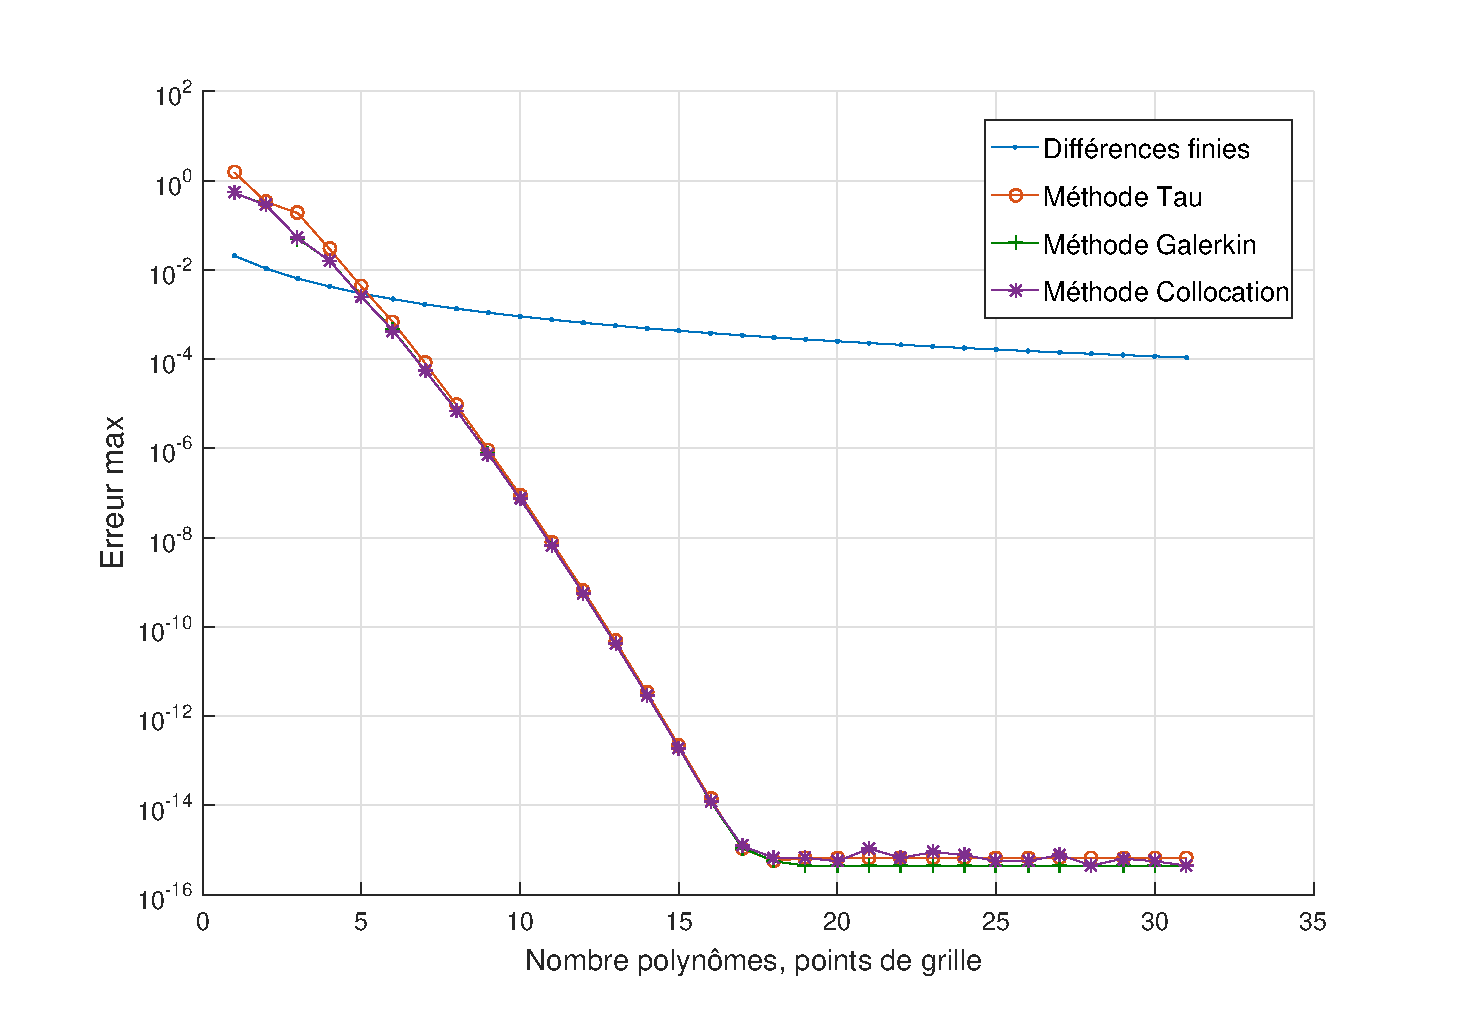
\includegraphics[width=13cm]{graphe_erreur.eps}
  \caption{Comparaison selon méthode de l'erreur maximale avec la solutions analytique}
  \label{fig_erreur}
\end{figure}


 \part{Exercice sur l'équation de Schrödinger}
\setcounter{section}{0}
 
%\section{Introduction}


\section{équation de Schrödinger stationnaire}

\section{équation de Schrödinger dépendant du temps}

$$\dot{\imath}\hbar\frac{\partial}{\partial t}\ket{\Psi(t)}=\left[\frac{1}{2}p^2+ V(x)+A(t)p\right]\ket{\Psi(t)}\;.$$

avec

\begin{equation}
A(t)= A_{0}f(t-t_{0})\sin(\omega (t-t_{0}))
\end{equation}

on prend $t_{0}=0$

L'enveloppe :
$$f(t-t_{0})=\cos^{2} \left(\frac{\omega (t-t_{0})}{2k}\right)$$

pour $\frac{-\pi k}{\omega}<t-t_{0}<\frac{\pi k}{\omega}$.



\begin{equation}
\sum_{n=0}^{N}\phi_{n}(x)\dot{b}_{n}(t) e^{-iE_{n}t} = - A(t) \sum_{m=0}^{N}\frac{\partial \phi_{m}(x)}{\partial x}b_{m}(t) e^{-iE_{m}t}\;.
\end{equation}

on multiplie par $\phi_{n}^{\ast}(x) e^{iE_{n}t}$

On a 

\begin{equation}
\dot{b}_{n}(t) = - A(t) \int \sum_{m=0}^{N}\phi_{n}^{\ast}(x)\frac{\partial \phi_{m}(x)}{\partial x}b_{m}(t) e^{-i(E_{m}-E_{n})t} dx\;.
\end{equation}

où

\begin{equation}
I_{m,n}= \int \phi_{m}^{\ast}(x)\frac{\partial \phi_{n}(x)}{\partial x} dx\;.
\end{equation}
avec
\begin{equation}
\phi_{n}(x) = \sum_{k=0}^{N} a_{k,n}\varphi_{k}(x)\;.
\end{equation}

c'est parti :
\begin{equation}
\phi_{m}^{\ast}(x)\frac{\partial \phi_{n}(x)}{\partial x} = \sum_{k=0}^{N} a_{k,m}^{\ast}\varphi_{k}^{\ast} \cdot \left(\sum_{l=1}^{N}a_{l,n} \sqrt{\frac{l}{2}}\varphi_{l-1}(x)-\sum_{l=0}^{N-1}a_{l,n}\sqrt{\frac{l+1}{2}}\varphi_{l+1} \right)\;.
\end{equation}

avec 

\begin{equation}
\varphi'_{l}(x) =  \sqrt{\frac{l}{2}} \varphi_{l-1}(x)-\sqrt{\frac{l+1}{2}}\varphi_{l+1}(x)\;.
\end{equation}

On a après intégration (relation orthogonalité des fonctions d'Hermites) et en posant $l =k+1$ dans premier terme de la parenthèse et $l =k-1$ dans le second :

\begin{equation}
I_{m,n} = \sum_{k=0}^{N-1} a_{k,m}^{\ast}  a_{k+1,n} \sqrt{\frac{k+1}{2}}- \sum_{k=1}^{N} a_{k,m}^{\ast}a_{k-1,n}\sqrt{\frac{k}{2}}\;.
\end{equation}

pour $m,n = 0,1,..,N$. Où l'on peut remarquer que la première somme termine à $N-1$ et la seconde commence à $1$, car $k =0,1,..,N$ doit être respecté.




On implémente cette fonction dans Matlab avec Ode15s pour trouver les $b(t)$ :

\begin{equation}
\dot{b}_{m}(t) = - A(t) \sum_{n=0}^{N}I_{m,n}b_{n}(t) e^{-i(E_{m}-E_{n})t}\;.
\end{equation}
pour $m=0,..,N$.

on aura sous forme matricielle :

\begin{equation}
\frac{d}{dt}
\begin{pmatrix}
 b_{0}\\ 
 b_{1}\\ 
 \vdots\\ 
 b_{N-1}\\ 
  b_{N}
\end{pmatrix} = -A(t) \cdot M(t) \cdot 
\begin{pmatrix}
 b_{0}\\ 
 b_{1}\\ 
 \vdots\\ 
 b_{N-1}\\ 
  b_{N}
\end{pmatrix}\;.
\end{equation}

où $M(t)$ est le produit d'Hadamard (commande Matlab : .*) des matrices $I_{m,n}$ et $e^{-i(E_{m}-E_{n})t}$. 

On prend conditions initiales : $b_{0}=1$ et $b_{n}=0$ pour $n > 0$. Etat initial dans le fondamental.


\subsection{résultats}

Calculons 

$$\left| b_{0}(t)\right|^2= b^\ast_0(t)b_0(t)$$

$$\left| b_{1}(t)\right|^2= b^\ast_1(t)b_1(t)$$

 
or
$$\sum_{n} \left| b_{n}(t)\right|^2 =1$$

donc probabilité d'ionisation :

$$1-\left| b_{0}(t)\right|^2-\left| b_{1}(t)\right|^2$$

graphes avec proba état ds les 2 états et

la probabilité d'ionisation en fonction de  $w$ .



Si $w$ est egale différence d'energie , c'est à dire résonance.

regarder proba de rester ds etat fondamental en fonction du temps et d'etre ds état ionisation en fonction du temps.

Normalement les 2 courbles oscille en opposition de phase.  c'est oscillations de rabi

%\section*{Conclusion}


\end{document}
